\newcommand{\conjuntoItens}{

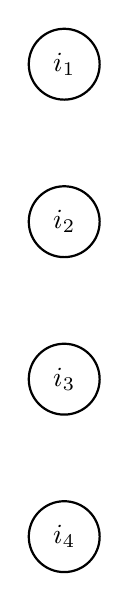
\begin{tikzpicture}[
    thick,
    item/.style={circle, draw, minimum size=9mm},
    buyer/.style={circle, draw,  minimum size=9mm}
]
    % Itens
    \node[item] (i1) at (0,2) {$i_1$};
    \node[item] (i2) at (0,0) {$i_2$};
    \node[item] (i3) at (0,-2) {$i_3$};
    \node[item] (i3) at (0,-4) {$i_4$};

\end{tikzpicture}
}


\newcommand{\conjuntoCompradores}{

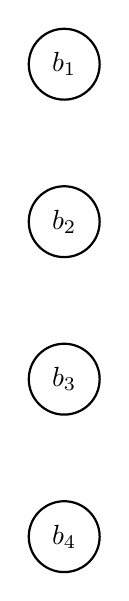
\begin{tikzpicture}[
    thick,
    item/.style={circle, draw, minimum size=9mm},
    buyer/.style={circle, draw,  minimum size=9mm}
]

    % Compradores
    \node[buyer] (b1) at (5,2) {$b_1$};
    \node[buyer] (b2) at (5,0) {$b_2$};
    \node[buyer] (b2) at (5,-2) {$b_3$};
    \node[buyer] (b2) at (5,-4) {$b_4$};

\end{tikzpicture}
}


\newcommand{\conjuntoItensValorados}{

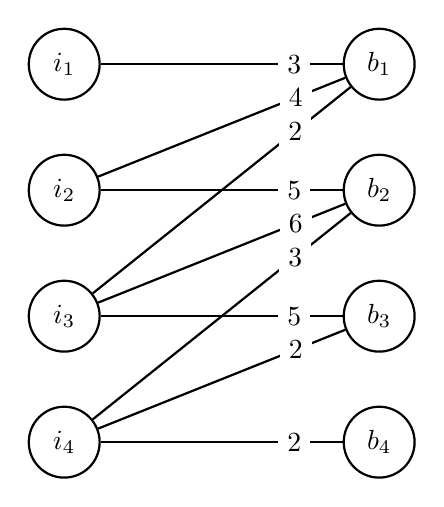
\begin{tikzpicture}[
    thick,
    item/.style={circle, draw, minimum size=9mm},
    buyer/.style={circle, draw,  minimum size=9mm},
    scale=0.8
]
    % Itens
    \node[item] (i1) at (0,2) {$i_1$};
    \node[item] (i2) at (0,0) {$i_2$};
    \node[item] (i3) at (0,-2) {$i_3$};
    \node[item] (i4) at (0,-4) {$i_4$};

    % Compradores
    \node[buyer] (b1) at (5,2) {$b_1$};
    \node[buyer] (b2) at (5,0) {$b_2$};
    \node[buyer] (b3) at (5,-2) {$b_3$};
    \node[buyer] (b4) at (5,-4) {$b_4$};

    % Arestas
    \draw (b1) --node[pos=0.2, fill=white]{3} (i1);
    \draw (b1) --node[pos=0.2, fill=white]{4} (i2);
    \draw (b1) --node[pos=0.215, fill=white]{2} (i3);

    \draw (b2) --node[pos=0.2, fill=white]{5} (i2);
    \draw (b2) --node[pos=0.2, fill=white]{6} (i3);
    \draw (b2) --node[pos=0.215, fill=white]{3} (i4);

    \draw (b3) --node[pos=0.2, fill=white]{5} (i3);
    \draw (b3) --node[pos=0.2, fill=white]{2} (i4);

    \draw (b4) --node[pos=0.2, fill=white]{2} (i4);
    % \draw (i2) -- (b2);
    % \draw (i3) -- (b2);
\end{tikzpicture}
}

\newcommand{\conjuntoItensPrecificados}{

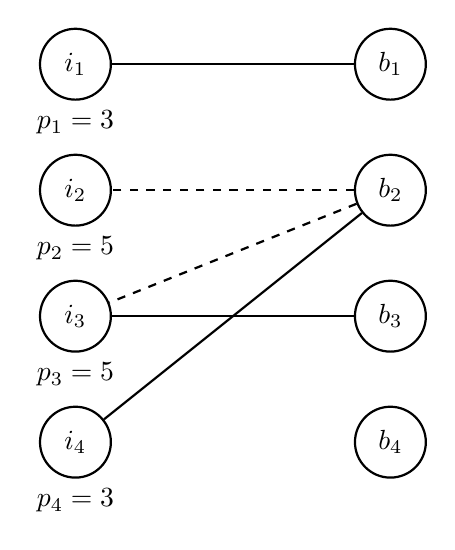
\begin{tikzpicture}[
    thick,
    item/.style={circle, draw, minimum size=9mm},
    buyer/.style={circle, draw,  minimum size=9mm},
    scale=0.8
]
    % Itens
    \node[item, label=below:{$p_1 = 3$}] (i1) at (0,2) {$i_1$};
    \node[item, label=below:{$p_2 = 5$}] (i2) at (0,0) {$i_2$};
    \node[item, label=below:{$p_3 = 5$}] (i3) at (0,-2) {$i_3$};
    \node[item, label=below:{$p_4 = 3$}] (i4) at (0,-4) {$i_4$};

    % Compradores
    \node[buyer] (b1) at (5,2) {$b_1$};
    \node[buyer] (b2) at (5,0) {$b_2$};
    \node[buyer] (b3) at (5,-2) {$b_3$};
    \node[buyer] (b4) at (5,-4) {$b_4$};

    % Arestas
    \draw (i1) -- (b1);
    \draw (i4) -- (b2);
    \draw (i3) -- (b3);


    % \draw[dashed, thick] (b1) -- (i2);
    % \draw[dashed, thick] (b1) -- (i3);

    \draw[dashed, thick] (b2) -- (i2);
    \draw[dashed, thick] (b2) --(i3);

    % \draw[dashed, thick] (b3) --(i4);

    % \draw[dashed, thick] (b4) -- (i4);
    
\end{tikzpicture}
}


\newcommand{\fluxograma}{
    \begin{tikzpicture}[
        every node/.style={draw, minimum height=1.2cm, minimum width=3.8cm, font=\ttfamily, align=center},
        decision/.style={aspect=2, draw, minimum height=1.5cm, inner sep=0pt},
        arrow/.style={->, thick},
        node distance=1.2cm and 2cm
    ]
        % Nós
        \node (begin) at (-10,-1.5) [circle, draw, minimum size=1.2cm] {Início};
        \node (genKeys) at (-5,-1.5) {Gerar a população\\ inicial};
        \node (fitness) at (-5, -4) {Avaliação de \\ fitness};
        \node (checkStop) at (4, -4) [diamond, decision, fill=gray!20] {Critério de parada\\ satisfeito?};
        \node (selection) at (4, -8) {Seleção};
        \node (crossover) at (-1.5, -8) {Cruzamento};
        \node (mutation) at (-7.5, -8) {Mutação};
        \node (elitism) at (-13.5, -8) {Elitismo};
        \node (newPop) at (-13.5, -4) {Nova população};
        \node (final) at (4, -1) [circle, draw, minimum size=1.2cm] {Fim};
        
    \begin{scope}[
              every node/.style={fill=white,circle}, arrow/.style={->,ultra thick}]
        % Conexões
        \draw[arrow] (begin) -- (genKeys);
        \draw[arrow] (genKeys) -- (fitness);
        \draw[arrow] (fitness) -- (checkStop);
        \draw[arrow] (checkStop) --node[right]{Não} (selection);
        \draw[arrow] (selection) -- (crossover);
        \draw[arrow] (crossover) -- (mutation);
        \draw[arrow] (mutation) -- (elitism);
        \draw[arrow] (elitism) -- (newPop);
        \draw[arrow] (newPop) -- (fitness);
        \draw[arrow] (checkStop) -- node[right]{Sim} (final);
        
    \end{scope}
    \end{tikzpicture}
}

\newcommand{\fluxogramaBRKGA}{
    \begin{tikzpicture}[
        every node/.style={draw, minimum height=1.2cm, minimum width=3.8cm, font=\ttfamily, align=center},
        decision/.style={aspect=2, draw, minimum height=1.5cm, inner sep=0pt},
        arrow/.style={->, thick},
        node distance=1.2cm and 2cm
    ]
        % Nós
        \node (begin) at (-10,-1.5) [circle, draw, minimum size=1.2cm] {Início};
        \node (genKeys) at (-5,-1.5) {Gerar os vetores\\ de chaves aleatórias};
        \node (fitness) at (-5, -4) {Decodificar cada vetor \\ de chave aleatória};
        \node (checkStop) at (4, -4) [diamond, decision, fill=gray!20] {Regra de parada\\ satisfeito?};
        \node (selection) at (4, -8) {Classificar indivíduos\\como elite ou não-elite};
        \node (crossover) at (-2, -8) {Copiar os elite para\\a próxima geração};
        \node (mutation) at (-7.5, -8) {Criar mutantes para\\próxima geração};
        \node (elitism) at (-13.5, -8) {Gerar descendentes para\\a próxima geração};
        \node (newPop) at (-13.5, -4) {Nova população};
        \node (final) at (4, -1) [circle, draw, minimum size=1.2cm] {Fim};
        
    \begin{scope}[
              every node/.style={fill=white,circle}, arrow/.style={->,ultra thick}]
        % Conexões
        \draw[arrow] (begin) -- (genKeys);
        \draw[arrow] (genKeys) -- (fitness);
        \draw[arrow] (fitness) -- (checkStop);
        \draw[arrow] (checkStop) --node[right]{Não} (selection);
        \draw[arrow] (selection) -- (crossover);
        \draw[arrow] (crossover) -- (mutation);
        \draw[arrow] (mutation) -- (elitism);
        \draw[arrow] (elitism) -- (newPop);
        \draw[arrow] (newPop) -- (fitness);
        \draw[arrow] (checkStop) -- node[right]{Sim} (final);
        
    \end{scope}
    \end{tikzpicture}
}
